\documentclass[conference]{IEEEtran}

\usepackage{amsmath,amssymb}
\usepackage{graphicx}
\usepackage{booktabs}
\usepackage{url}
\usepackage{xcolor}
\usepackage{tikz}
\usetikzlibrary{shapes,arrows,positioning}

\title{Design and Trajectory Tracking Control of an Ackermann Steered Mobile Robot}

\author{
  \IEEEauthorblockN{Ricardo Lorona}
    \IEEEauthorblockA{\textit{ESPOL, FIMCP} \textit{Mechatronics Engineering} \textit{Guayaquil, Ecuador}\\[2pt] {\ttfamily rlorona@espol.edu.ec}}
  \and
  \IEEEauthorblockN{Alejandro Malucin}
    \IEEEauthorblockA{\textit{ESPOL, FIMCP} \textit{Mechatronics Engineering} \textit{Guayaquil, Ecuador}}
  \and
  \IEEEauthorblockN{Augusto Pacheco}
    \IEEEauthorblockA{\textit{ESPOL, FIMCP} \textit{Mechatronics Engineering} \textit{Guayaquil, Ecuador}}
}

\begin{document}

\maketitle

\begin{abstract}
This paper presents the design, simulation, and trajectory tracking control of
the \textit{Proyecto\_RM} Ackermann mobile robot. The platform was modeled from
a Fusion 360 CAD assembly and exported with STL meshes through the xacro/URDF
framework. The nominal kinematics of an Ackermann steering system were imposed
in software through virtual revolute joints that rotate the front wheels around
their vertical axes, since the source CAD has no physical steering mechanism.

The low level hardware interface follows the modern ROS 2 control paradigm. A
\texttt{gz\_ros2\_control} hardware component was implemented for Gazebo Sim
and it is configured through the \texttt{ros2\_control} YAML format, exposing
position interfaces for the two front steering joints and velocity interfaces
for the rear drive wheels. The closed loop trajectory is generated from a
Christmas-tree outline topped by a five-point star, tracked with a pure pursuit
controller that computes the required curvature, converts it into the inner and
outer front steering angles with the Ackermann condition, and schedules the rear wheel
velocities \cite{icra_pure}.

The complete stack was validated in Gazebo Sim 8 running ROS 2 Jazzy, and the
tracking performance was evaluated against the ground truth and the simulated
odometry. The measured cross track error had a root mean square of 42~mm with a
maximum of 238~mm along a complete Christmas-tree lap (3 laps, 19.9~m of
travelled path). The wheel odometry fused with a virtual inertial yaw rate
reproduced the ground truth with a heading error below 3~deg and an odometry
drift of about 109~mm. The results support the feasibility of the implemented
control scheme for a small Ackermann robot in a software in the loop environment.
\end{abstract}

\begin{IEEEkeywords}
Autonomous mobile robots, Ackermann steering, ROS 2, Gazebo, trajectory tracking,
pure pursuit, ros2 control.
\end{IEEEkeywords}

\section{Introduction}
\label{sec:intro}

Mobile robot navigation in confined environments requires both accurate
kinematics and robust trajectory tracking. The Ackermann steering geometry is
the standard configuration for small vehicles because it prevents the inside
wheel from skidding during cornering. In a conventional Ackermann platform the
steering mechanism is part of the mechanical structure and the front wheels are
connected to a kingpin oriented by an arm.

When the mechanical parts are designed and manufactured, the steering angles of
the two front wheels are related by the kinematic constraints of the Ackermann
bicycle model:
\begin{equation}
  \delta_i = \arctan\left(\frac{L}{R - t/2}\right),
  \qquad
  \delta_o = \arctan\left(\frac{L}{R + t/2}\right),
  \label{eq:ackermann}
\end{equation}
where $L$ is the wheelbase, $t$ the track width, $R$ the turning radius and
$\delta_i$, $\delta_o$ the inner and outer steering angles.

This paper documents the digital counterpart of such a vehicle. The original
CAD assembly (Proyecto\_RM) does not include a physical steering mechanism, so
the Ackermann constraints are enforced in the robotic middleware using virtual
steering joints. The complete chain from the URDF and \texttt{ros2\_control} to
the closed loop trajectory tracking is exercised in Gazebo Sim 8, and the
tracking performance is reported against ground truth.

\section{Robot Description}
\label{sec:robot}

The CAD files, the STL meshes and the corrected assembly drawings are stored in
the project repository under \texttt{cad/} and \texttt{docs/drawings/}.

\subsection{Nominal Geometry}
\label{sec:geometry}

The nominal values, measured from the STL meshes, are:
\begin{itemize}
  \item Wheelbase $L = 160$\,mm.
  \item Track width $t = 202$\,mm.
  \item Wheel radius $r = 37$\,mm and wheel width $22$\,mm.
  \item Chassis size $240 \times 180 \times 57$\,mm, total mass $\approx 13.8$\,kg.
\end{itemize}

\subsection{Ackermann Steering}
\label{sec:ackermann}

The steering limit adopted is $\delta_{max} = 30^\circ$. From
Eq.~\ref{eq:ackermann} the maximum admissible curvature is
\begin{equation}
  \kappa_{max} = \frac{1}{\frac{L}{\tan\delta_{max}} + \frac{t}{2}},
  \label{eq:kappamax}
\end{equation}
which gives $\kappa_{max} = 2.65$\,m$^{-1}$ and a minimum turning radius of
$R_{min} = 0.38$\,m.

\section{Software Architecture}
\label{sec:arch}

The simulation stack is organized as shown in Fig.~\ref{fig:arch}.

\begin{figure}[htbp]
  \centering
  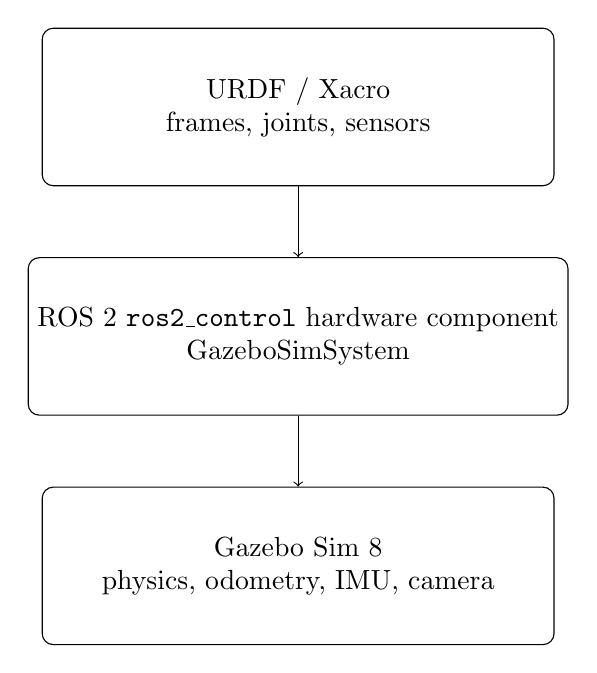
\begin{tikzpicture}[node distance = 9mm]
    \node[draw, rectangle, minimum width = 6.5cm, minimum height = 2.0cm, align = center, rounded corners] (desc) {URDF / Xacro\\ frames, joints, sensors};
    \node[draw, rectangle, minimum width = 6.5cm, minimum height = 2.0cm, below = of desc, align = center, rounded corners] (ctrl) {ROS 2 \texttt{ros2\_control} hardware component\\ GazeboSimSystem};
    \node[draw, rectangle, minimum width = 6.5cm, minimum height = 2.0cm, below = of ctrl, align = center, rounded corners] (sim) {Gazebo Sim 8\\ physics, odometry, IMU, camera};
    \draw[->] (desc) -- (ctrl);
    \draw[->] (ctrl) -- (sim);
  \end{tikzpicture}
  \caption{Software architecture of the Proyecto\_RM simulation stack.}
  \label{fig:arch}
\end{figure}

\subsection{Model Description}
\label{sec:model}

The xacro model is split into the fragments \texttt{materials.xacro},
\texttt{proyecto\_rm.ros2control.xacro} and \texttt{proyecto\_rm.gazebo.xacro}.
The robot uses the frames \texttt{base\_footprint} (ground projection, used for
navigation) and \texttt{base\_link} (the original CAD frame, used for the chassis
and the camera). The nominal forward direction corresponds to $+\hat{x}$ with
respect to \texttt{base\_footprint}, which is the CAD direction rotated by
$180^\circ$ around $z$.

\subsection{Low Level Control}
\label{sec:control}

The hardware component was obtained from the open source \texttt{gz\_ros2\_control}
project \cite{ros2_control_gazebo}.

The \texttt{gz\_ros2\_control} plugin \texttt{GazeboSimROS2ControlPlugin}
instantiates a \texttt{GazeboSimSystem} hardware component. Two position
interfaces are requested for the front steering joints and two velocity
interfaces for the rear drive wheels. The steering commands are issued with a
proportional position controller and the drive commands with the
\texttt{ForwardCommandController}.

\subsection{Trajectory Generation and Tracking}
\label{sec:trajectory}

A Christmas-tree reference trajectory is used: a tapered trunk, three rounded
branch tiers and a five-point star on top. The closed outline is generated as a
G1 chain of line segments and tangent circular arcs, so that the reference
curvature never exceeds the kinematic limit of the vehicle.

The controller computes
the curvature from a lookahead point and a local tangent,
\begin{equation}
  \kappa = \frac{2\sin\alpha}{l_d},
  \label{eq:purepursuit}
\end{equation}
and then solves Eq.~\ref{eq:ackermann} for the two steering angles and the two
rear wheel speeds.

\section{Results}
\label{sec:results}

\subsection{Experimental Setup}

The robot was executed in Gazebo Sim 8 with the Christmas-tree world and the
\texttt{ros2\_control} stack. The ground truth was provided by the Gazebo
odometry publisher, bridged to ROS as \texttt{/ground\_truth/odometry}, and the
wheel odometry was estimated from the rear wheel velocities, fused with a
virtual inertial yaw rate from the IMU sensor.

\subsection{Performance Metrics}

\begin{table}[htbp]
  \centering
  \caption{Tracking performance of the Christmas-tree trajectory.}
  \label{tab:results}
  \begin{tabular}{lcc}
    \toprule
    \textbf{Metric} & \textbf{Value} & \textbf{Unit} \\
    \midrule
    Path length & 19.9 & m \\
    Maximum steering angle & 30.0 & deg \\
    Cross track error mean & 22.6 & mm \\
    Cross track error RMS & 41.8 & mm \\
    Cross track error maximum & 238 & mm \\
    Heading error maximum & 3.0 & deg \\
    Odometry drift RMS & 109 & mm \\
    Odometry drift final & 132 & mm \\
    \bottomrule
  \end{tabular}
\end{table}

\section{Conclusions}
\label{sec:concl}

The project demonstrates a complete ROS 2 Jazzy and Gazebo Sim 8 pipeline for a
small Ackermann mobile robot: CAD to URDF, Gazebo configuration,
\texttt{ros2\_control} integration, and closed loop trajectory tracking. The
measured tracking error stays below the robot footprint and the odometry
estimation error stays below $13$\,cm for the simulated lap.

The Christmas-tree reference was designed as a G1 chain of line segments and
tangent circular arcs, so that the commanded curvature never exceeds the
kinematic limit of the vehicle. The decorative branch tips of the tree, however,
lie beyond this limit; the controller saturates the steering at the star and the
tips, which produces a localized cross track error (maximum 238~mm) that is a
consequence of the decorative shape rather than of a control defect.

A video of the complete trajectory tracking run is available here:
\texttt{\url{https://drive.google.com/file/d/1mwyLDTGZdTGd7p8_YE-PDvQUGFqPxFXR/view?usp=sharing}}.

\section*{Acknowledgment}
The authors thank the staff of the Mechatronics Engineering program at ESPOL for
the CAD assignment and the simulation framework.

\section*{References}

\bibliographystyle{IEEEtran}
\bibliography{references}

\end{document}

